\section{Results}
\paragraph{Throughout the relevance and development phases\todo{consider changing phase labels as noted in methods section}, the CHVs and nurses emphasized three key priorities for the design of a potential patient management system: communication from the CHV to the clinic, communication between the clinic and the CHV, and reminders for CHVs to help them keep up with their myriad of responsibilities on a day to day basis.} 

\subsection{From CHV to Clinic}
\subsubsection{Reporting Home Visits}
\paragraph{CHVs described conducting home visits with patients as their major responsibility. They made rounds in their village at least one day per week, depending on their own work schedules. Number of households visited varied per week, but participants in the focus group collectively concluded that it took approximately 5-6 months to complete rounds at every household in their village before beginning again. Every two weeks, CHVs were required to visit the health facility to submit reports detailing a number of demographics - including number of pregnant women, number of infants under six months of age, number of children under age five, number of births, and number of women provided with family planning information and materials. These reports are then compiled for each month by the CHEWs\todo{i think this is the first this appears. introduce earlier, but even then, i suggest replacing acronym with the word supervisor.} of each region. Members of the focus group were unable to describe what type of analysis or evaluation took place after submission of their reports, and some questioned whether any oversight of the reported data took place.\todo{modify this description by deleting the part after the comma}}

Table~\ref{tab:chvreport}
\begin{table}[]
  \centering
  \caption{Selected indicators from June 2013 CHV Monthly Report}
    \begin{tabular}{lrrr}
    \toprule
    \textbf{Community Unit} & \textit{Sinoko} & \textit{Magemo} & \textit{Sitabicha} \\
    \midrule
    Households & 148   & 6     & 92 \\
    Pregnant women & 22    & 9     & 8 \\
    Pregnant women who did not attend at least 4 ANC visits & 19    & 1     & 7 \\
    Pregnant women referred & 15    & 5     & 3 \\
    Deliveries by unskilled birth attendants & 11    & 3     & 7 \\
    Births & 30    & 4     & 10 \\
    Newborns referred & 17    & 4     & 10 \\
    Women aged 25-49 provided with FP commodities & 58    & 2     & 10 \\
    Maternal deaths & 0     & 0     & 0 \\
    \bottomrule
    \end{tabular}%
  \label{tab:chvreport}%
\end{table}%


\paragraph{During field visits \todo{consider a different name of activity as mentioned earlier}with the research team, the CHVs described the reporting process as difficult and somewhat disjointed. Both CHVs observed took minimal notes when making home visits, instead opting to complete their log sheets at the end of the day\todo{do we know why?}. During the field visit days, the CHVs and research team met with four and five households respectively. Time spent at each household varied based on the family's concerns and size of the family, but lasted anywhere from fifteen minutes to one hour. Both CHVs carried 'referral books', which contained a series of carbon-copied sheets with spaces for the date, patient name, and chief complaint to be completed by the CHV. Each sheet had three copies: one for the CHV, one for the patient, and one to be kept at the clinic. However, both CHVs indicated that they rarely kept their copy of the referral sheets\todo{any insight into why...e.g., no way to keep records?} and were unable to show the research team any sheets from previous referrals.}

\paragraph{Discussion with the clinic nurses offered additional insight into the nature of CHV home visits. They noted that the CHVs submitted reports that were compiled monthly by the CHEWs. However, the nurses indicated that they rarely looked at the monthly CHV log books to track patient visits. Instead, the main indication of CHVs conducting home visits was the presence of patients with referral slips from their CHVs. The nurses reported that they received approximately 50 CHV referrals per week\todo{meaning slips? seems high for actual slips. if correct, let's put in terms of weekly patient volume}, with an estimated 15 being related to antenatal care visits. They also indicated that patients rarely came in with both copies of the CHV referral sheets, making it difficult to completely track the flow of referrals from CHV to clinic accurately.}

\paragraph{Based on these findings, the research team designed a fast and simple method of reporting home visits to pregnant women and new mothers within a Verboice call flow. After completing a visit, the CHV flashes\todo{have you described this? include in the methods section} the Baby Monitor number and receives a free incoming call from the system. After indicating that they are a CHV and identifying themselves with their unique ID number, they are asked to \todo{to select from a menu of options that includes reporting a home visit}confirm that they would like to report a home visit. They are subsequently asked to identify the household they have visited by \todo{entering the phone number the woman provided at enrollment...we also need to describe somewhere how the CHV gets the woman's number.} their phone number. After confirming the phone number, they are asked to indicate the date of the visit by pressing '1' for today, '2' for yesterday, and '3' for another date\todo{before yesterday}. If they select another date, they are asked to input the month and date (following separate prompts) using their keypads. This information is saved in the Baby Monitor database, and the call is completed.}

Fig ~\ref{fig:homevisit}.
\begin{figure}[]
	\begin{center}
	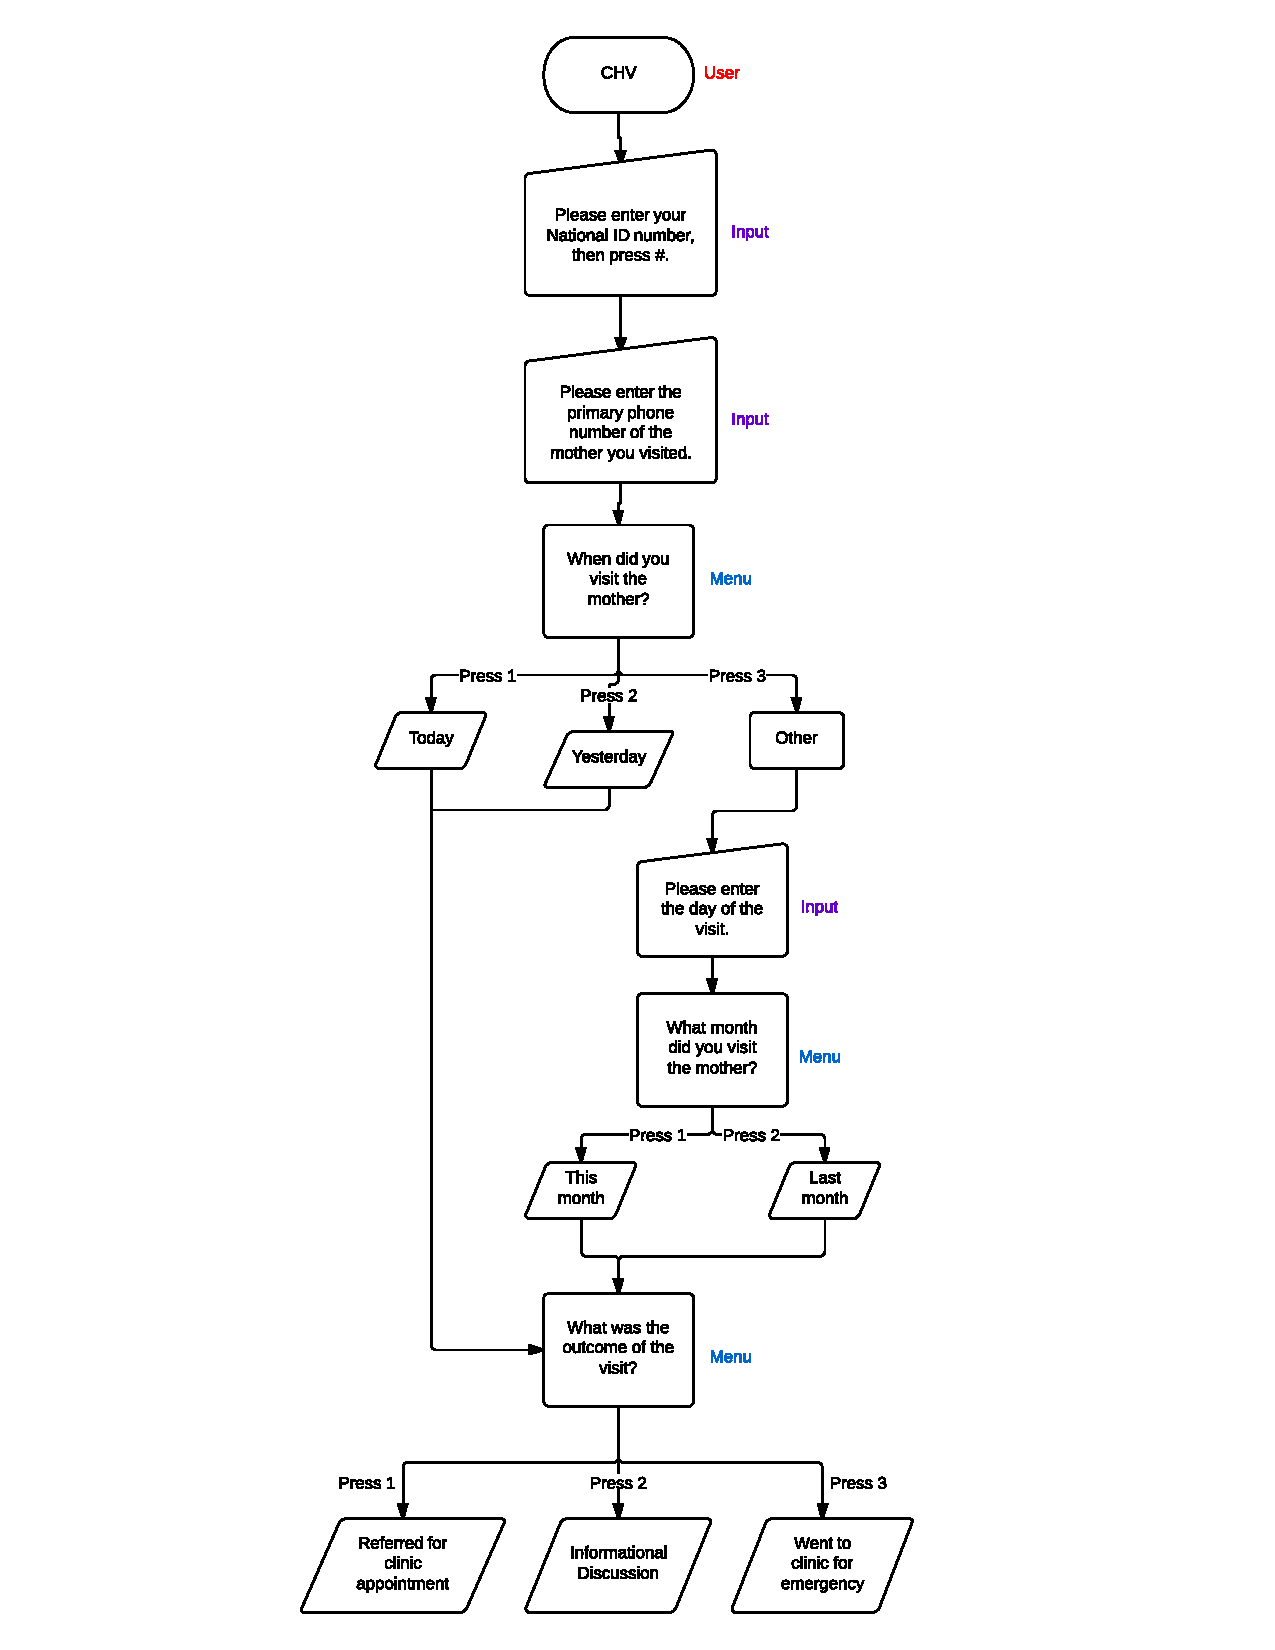
\includegraphics[height=8.3in, width=6.2in]{report-home-visit}
	\end{center}
	\caption{Call flow for reporting a home visit.}
	\label{fig:homevisit}
\end{figure}

\subsubsection{Reporting Home Deliveries}
\paragraph{As expected, both the CHV and nurse focus groups indicated that most pregnant women in this region delivered at home. Some of these women opt to deliver with their CHVs present, but many also use the services of birth attendants who assist in the delivery process in the woman's home. CHVs indicated little trouble in identifying home deliveries for reporting, as word of a new birth usually spread through the village quickly. The CHVs emphasized that word of mouth and speaking with community members was an especially important way for them to identify individuals who may require care. On the first field visit day with the research team, the CHV visited two new mothers after hearing from another community member that they had given birth within the past two months. Although the CHVs acknowledged a potential time delay in identifying deliveries by word of mouth, they collectively agreed that most deliveries were reported relatively soon after taking place.}\todo{within the first day? need to be more specific here. cases observed are very late. even best case scenario might be outside of window when most maternal and neonatal deaths occur.} 

\paragraph{The clinic nurses indicated that the only report of home deliveries they receive are on the CHV monthly reports, which they previously acknolwedged to using very rarely. They attributed the preference to deliver at home to cost of travel to Sinoko, and also indicated that not regularly checking for the number of recent deliveries presents challenges for providing postnatal care to women and children who may need it at the clinic.}

\paragraph{To address these findings, the research team designed a call flow similar to that of reporting CHV home visits for reporting deliveries. After flashing the Baby Monitor system and identifying themselves as CHVs, the CHV is asked to identify the woman who has delivered by her phone number. Date of delivery is indicated by pressing '1' for today, '2' for yesterday, and '3' for another date, which is input directly using their keypads. This delivery information is saved into the Baby Monitor database, and the call is completed.}

Fig ~\ref{fig:delivery}.
\begin{figure}[]
	\begin{center}
	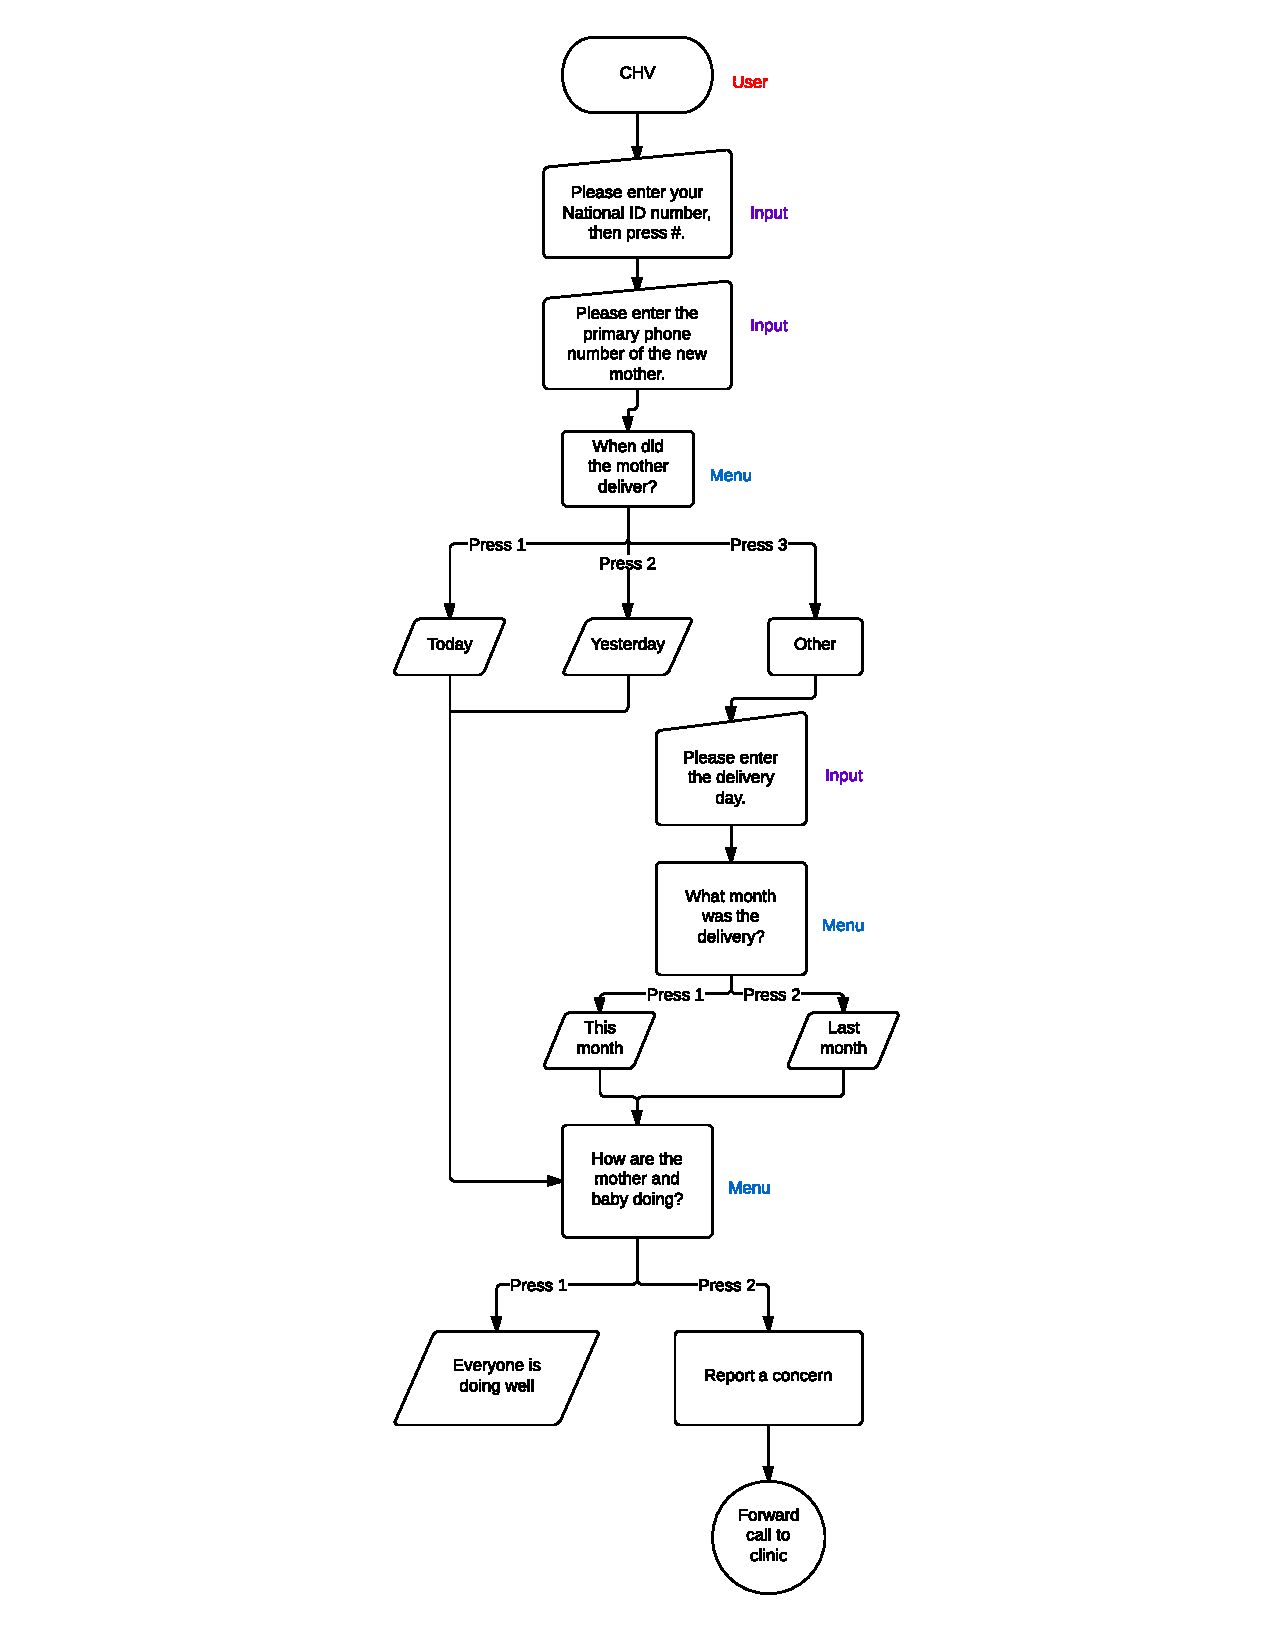
\includegraphics[height=8.3in, width=6.2in]{report-delivery}
	\end{center}
	\caption{Call flow for reporting a delivery.}
	\label{fig:delivery}
\end{figure}

\subsubsection{Reporting Emergencies}
\paragraph{The CHV focus group identified emergency reporting as a major area of concern in their existing workflow. CHVs reported that they were usually called by a family member during a health-related or pregnancy-related emergency. In most cases, they recommended that the patient travel to Sinoko\todo{i'd refrain from using the clinic name throughout this document, even in the setup section} to receive care at the clinic. However, they noted numerous occasions in which the patient arrived at Sinoko, only to find the clinic understaffed at that time of day or unprepared to handle certain emergency procedures due to limited medical supplies. The group attributed this to a lack of direct communication between the CHVs and the clinic, indicating if they knew that the clinic was not prepared for an incoming patient, they could refer and accompany the patient to another clinic or Webuye District Hospial\todo{same here. refer to closest level 3 facility}. They also indicated that news of these missed emergencies contributed to an unwillingness to visit Sinoko among community members. This perception was reflected during both field visit dates, as three separate pregnant women expressed some concern about delivering at Sinoko due to a combination of cost and prior missed emergencies.}

\paragraph{Discussion with the clinic nurses also reflected concerns about emergency reporting and referral to the clinic. The nurses acknowledged that there was little to no direct communication between CHVs and the clinic staff about incoming emergencies. Pregnant women often came to deliver with little prior notice at any time of the day, making it difficult for the nurses to prepare for their care. The nurses indicated that only one nurse is typically on call overnight, and at least two nurses are needed to complete a safe delivery procedure. Moreover, the nurses indicated that the clinic has capacity for only three deliveries per week due to limited supplies. If more than three women came into the clinic for a delivery, they would have to wait for an ambulance to arrive from Webuye to take them to the District Hospital in town.}

\paragraph{Based on these results, the research team designed a simple call flow to be used by patients, family members of patients, and CHVs to report an emergency to a nurse on staff at Sinoko clinic. The user flashes the Baby Monitor system, and indicates that they would like to report an emergency. After confirming that the user would like to speak directly to a clinic nurse, the system forwards the call to the clinic phone, free of charge to the user. The user can then describe the emergency to the nurse at the clinic, and the nurse can advise the patient, family member, or CHV on how to proceed. This allows the nurse to prepare for the arrival of the patient and call the other nurses to the clinic if necessary.}

Fig ~\ref{fig:emergency}.
\begin{figure}[tbp]
	\begin{center}
	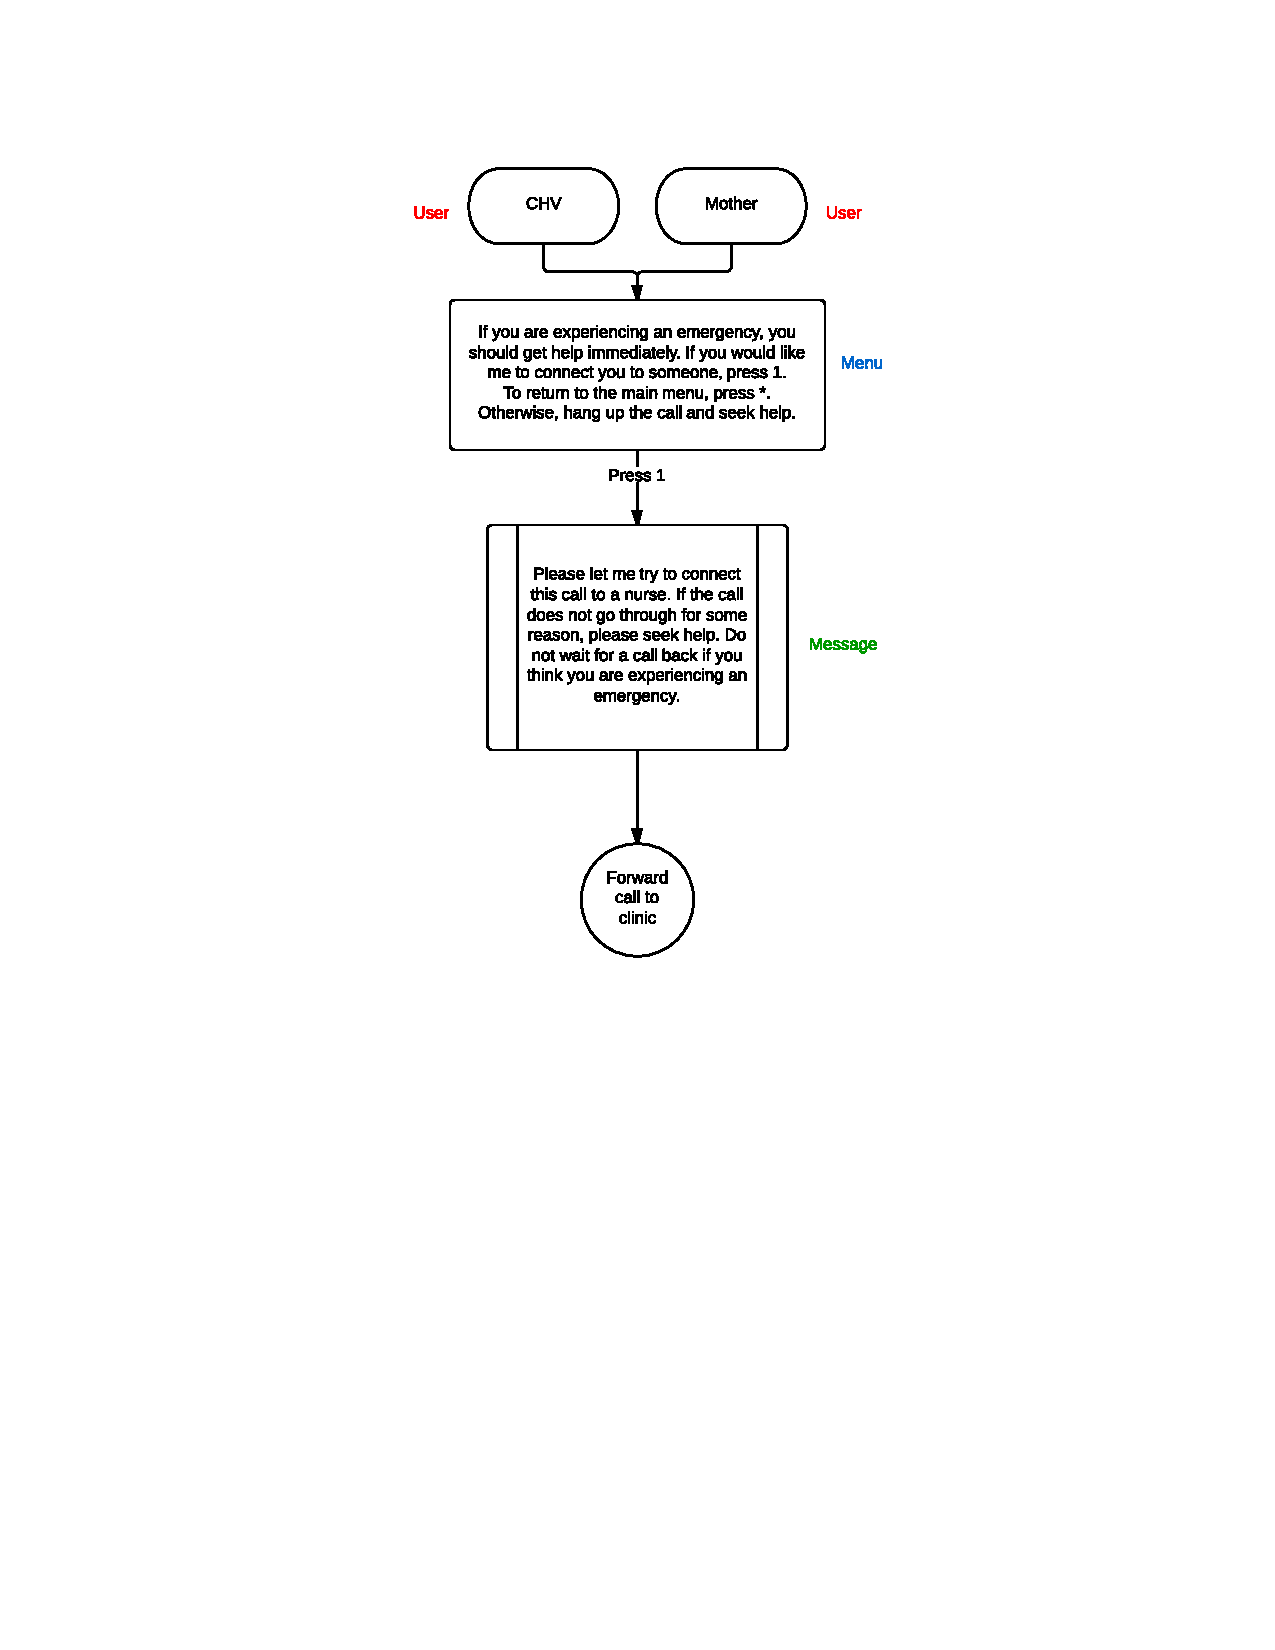
\includegraphics[height=8.3in, width=6.2in]{report-emergency}
	\end{center}
	\caption{Call flow for reporting an emergency.}
	\label{fig:emergency}
\end{figure}

\subsection{From Clinic to CHV}
\subsubsection{Clinic Visit Notifications}
%- as it was before the system
%- what the system adds

\subsubsection{Clinic Delivery Notifications}
%- as it was before the system
%- what the system adds

\subsection{Daily Reminders}
\subsubsection{Upcoming Home Visits}
%mock testing results

\subsubsection{Upcoming Delivery Dates}
%mock testing results


\subsection{Evaluation Outcomes}
\subsubsection{Usage of Patient Management System}
%To be determined; need to  write R script to analyze data for CHV use

\subsubsection{Usability Testing Results}
Fig ~\ref{fig:barchart}.
\begin{figure}[h]
	\begin{center}
	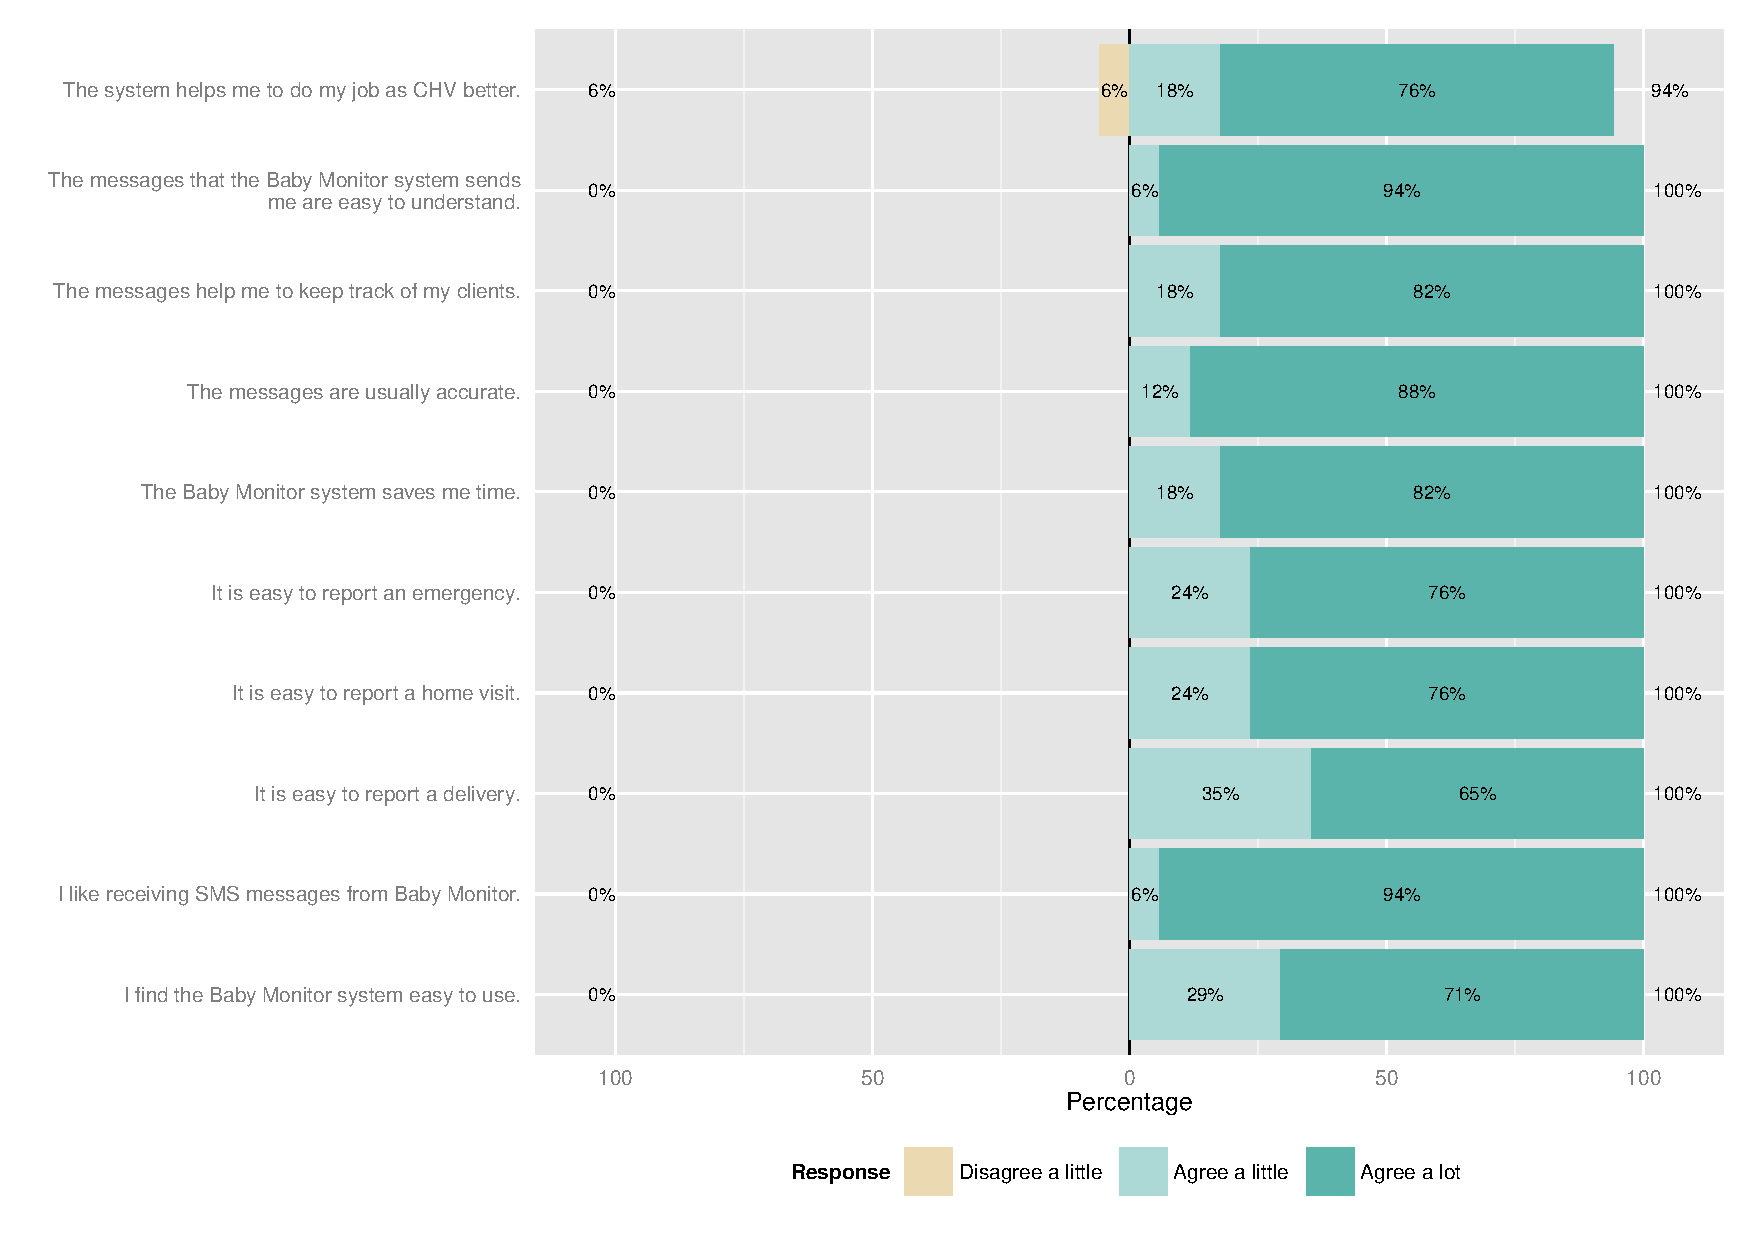
\includegraphics[height=4.5in]{usability-percent-grid}
	\end{center}
	\caption{CHVs generally found the service to be usable. The SMS messages sent by the system were among the highest rated features of the system. Overall, 94\% of respondents believed that the system helped them do their jobs as CHVs better than before.}
	\label{fig:barchart}
\end{figure}

